\documentclass[conference]{IEEEtran}

\usepackage{amsmath,amssymb}
\usepackage{booktabs}
\usepackage{graphicx}
\usepackage{url}

\title{On the Placement of RMS Normalization in Token Embedding Representations}

\author{
\IEEEauthorblockN{Tarun Balivada}
\IEEEauthorblockA{\textit{AI/ML Engineering Research}\\
India\\
GitHub: \url{https://github.com/professionaltarun2004/LLM-embeddings}}
}

\begin{document}
\maketitle

\begin{abstract}
Normalization can be applied to embedding vectors after lookup or to the rows of an embedding table before lookup. This paper asks whether these placements alter embedding geometry, fixed-table representations, or gradients with respect to a shared trainable table. Three controlled experiments use seeded synthetic embeddings and row-wise RMSNorm. In Experiment 0, the mean normalized-to-raw pairwise Euclidean distance ratio was 1.030494, while the maximum absolute cosine-similarity change was \(2.78\times10^{-16}\). In Experiment 1, lookup-then-normalize and normalize-table-then-lookup produced identical fixed-table representations. In Experiment 2, both paths produced the same loss (1.1457136942185433) and numerically equal, nonzero gradients for one deterministic mean-squared-error objective. These results are limited to the tested row-wise operation and synthetic data. No optimizer update, learned embedding, language task, or Transformer was evaluated.
\end{abstract}

\begin{IEEEkeywords}
RMSNorm, token embeddings, embedding geometry, normalization placement, gradient analysis
\end{IEEEkeywords}

\section{Introduction}
This investigation originated in a course/session discussion about incorporating normalization into an embedding representation rather than applying it after embedding lookup. The refined research question is:

\begin{quote}
What happens to the information and geometry of token embeddings when normalization is incorporated into the embedding representation itself, rather than applied after embedding lookup---and does the placement of normalization affect downstream model behavior?
\end{quote}

The experiments form a controlled progression. Experiment 0 measures geometric effects on a synthetic table. Experiment 1 compares two forward-computation arrangements for a fixed table. Experiment 2 compares gradients with respect to the same raw table under one scalar loss. The distinction between a raw table passed through normalization and a normalized representation used directly as the trainable parameter is central: only the former was tested.

\section{Background and Problem Formulation}
\subsection{Token IDs and Embedding Tables}
Let a vocabulary contain \(V\) token IDs, and let \(E\in\mathbb{R}^{V\times d}\) be an embedding table with dimension \(d\). An ID \(i\in\{0,\ldots,V-1\}\) selects row \(E_{i,:}\). Lookup selects vectors; it does not change token IDs or vocabulary. Throughout Experiments 0--2, \(E\) is synthetic and initialized by a seeded standard-normal draw. In Experiment 2, the table is marked trainable for differentiation, but no update is performed.

\subsection{Row-Wise RMSNorm}
For \(x\in\mathbb{R}^d\), the implemented normalization is
\begin{equation}
\operatorname{RMS}(x)=\sqrt{\frac{1}{d}\sum_{k=1}^{d}x_k^2},
\qquad
N_{\epsilon}(x)=\frac{x}{\max(\operatorname{RMS}(x),\epsilon)}.
\label{eq:rmsnorm}
\end{equation}
The experiments use \(\epsilon=10^{-8}\), reduce over the feature axis, and apply the same map independently to each row. No learned gain or bias is used.

\subsection{Normalization Placement}
For a token-ID sequence \(I=(i_1,\ldots,i_m)\), lookup is the row-selection operator \(L_I(E)\), with \([L_I(E)]_{t,:}=E_{i_t,:}\). Two paths are considered:
\begin{enumerate}
\item Lookup, then normalization: \(E[I]\rightarrow N_{\epsilon}\).
\item Normalize every table row, then lookup: \(N_{\epsilon,\mathrm{row}}(E)\rightarrow\) lookup.
\end{enumerate}
Both paths retain the raw table \(E\) as the underlying parameter. They do not test making a normalized representation itself the parameter.

\section{Mathematical Formulation}
Define \(N_{\epsilon,\mathrm{row}}(E)\) as applying Eq.~\eqref{eq:rmsnorm} independently to each row. The two outputs are
\begin{equation}
\begin{aligned}
Y_A(E,I)&=N_{\epsilon,\mathrm{row}}\!\left(L_I(E)\right),\\
Y_B(E,I)&=L_I\!\left(N_{\epsilon,\mathrm{row}}(E)\right).
\end{aligned}
\label{eq:paths}
\end{equation}
Equation~\eqref{eq:paths} formalizes the two placements compared in the experiments.
Because lookup selects rows and the same map acts independently on each row,
\begin{equation}
[N_{\epsilon,\mathrm{row}}(E)]_{i,:}=N_{\epsilon}(E_{i,:}),
\qquad
Y_B(E,I)_{t,:}=N_{\epsilon}(E_{i_t,:})=Y_A(E,I)_{t,:}.
\label{eq:commute}
\end{equation}
Thus the paths are algebraically identical under the stated row-local formulation. This reasoning does not cover normalization that mixes statistics across rows, uses different statistics at the two locations, or changes the parameterization. It is a mathematical property of this formulation; the experiments provide numerical checks for the implemented cases.

A third setup would optimize a normalized representation \(U\) directly, rather than optimize raw \(E\) and compute \(N_{\epsilon}(E)\). That is a different parameterization, with a different relation between the optimized variable and the effective embedding vectors. Experiments 0--2 do not evaluate it.

\section{Experimental Methodology}
\subsection{Experimental Controls}
Experiments 0 and 1 use seed 1729, vocabulary size 128, and dimension 32. Experiment 2 uses the same seeded initialization methodology and the same underlying tensor in both paths. All experiments use the same row-wise RMSNorm convention and epsilon. Experiment 1 uses token IDs 0--127; Experiment 2 uses \([3,17,42,91]\). No external corpus, pretrained embedding, optimizer, or Transformer is used.

\subsection{Metrics and Evaluation}
Experiment 0 evaluates all \(128\cdot127/2=8{,}128\) unique row pairs. Experiment 1 compares corresponding outputs and their pairwise geometry. Experiment 2 compares representations, scalar losses, and full gradients with respect to \(E\). Relative differences omit reference elements with magnitude at most \(10^{-12}\). Numerical equality checks use \(\mathrm{atol}=10^{-12}\) and \(\mathrm{rtol}=10^{-12}\).

\section{Experiment 0: Embedding Geometry}
\subsection{Setup}
A synthetic standard-normal \(128\times32\) matrix was generated using seed 1729. RMSNorm was applied independently to each row with \(\epsilon=10^{-8}\). The matrix is not a learned language-model embedding table.

\subsection{Results}
Table~\ref{tab:exp0} reports the pairwise measurements. Fig.~\ref{fig:distances} and Fig.~\ref{fig:cosines} show the saved comparisons.

\begin{table}[t]
\caption{EXPERIMENT 0: PAIRWISE GEOMETRY ON THE SYNTHETIC TABLE}
\label{tab:exp0}
\centering
\footnotesize
\setlength{\tabcolsep}{3pt}
\begin{tabular}{p{0.64\columnwidth}r}
\toprule
Measurement & Result\\
\midrule
Unique row pairs & 8,128\\
Mean row \(L_2\) norm, raw \(\rightarrow\) normalized & \(5.5091\rightarrow5.6569\)\\
Distance-ratio mean & 1.030494\\
Distance-ratio median & 1.021113\\
Distance-ratio standard deviation & 0.092586\\
Distance-ratio range & 0.817438--1.459170\\
Maximum absolute cosine change & \(2.78\times10^{-16}\)\\
\bottomrule
\end{tabular}
\end{table}

\begin{figure}[t]
\centering
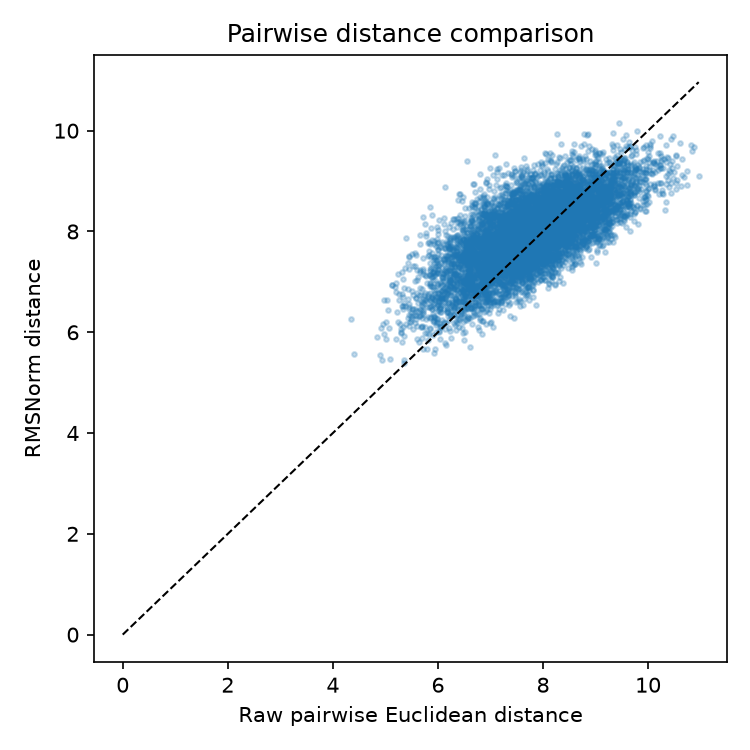
\includegraphics[width=0.92\columnwidth]{figures/pairwise_distances.png}
\caption{Experiment 0 pairwise Euclidean distances before and after RMSNorm. The diagonal denotes unchanged distances.}
\label{fig:distances}
\end{figure}

\begin{figure}[t]
\centering
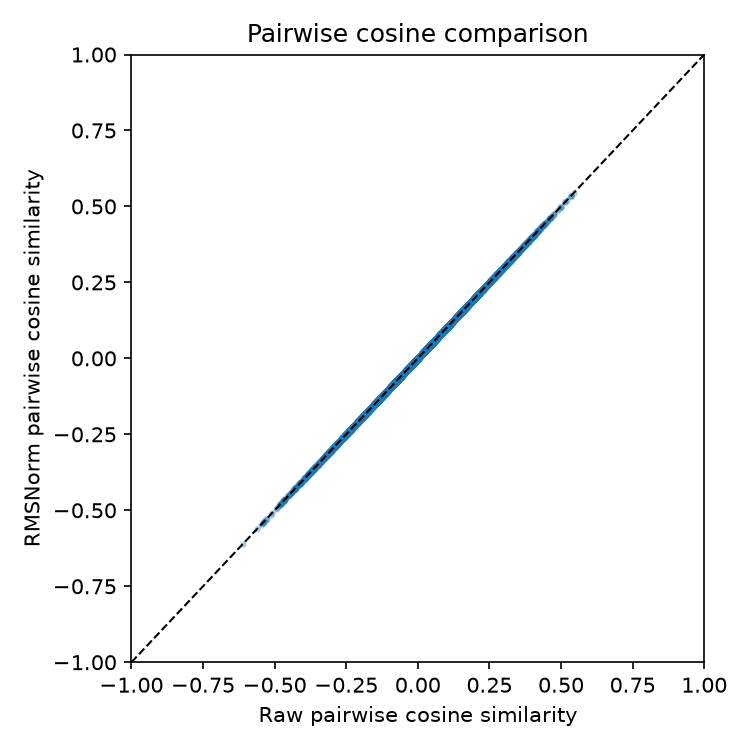
\includegraphics[width=0.92\columnwidth]{figures/pairwise_cosines.png}
\caption{Experiment 0 pairwise cosine similarities before and after RMSNorm. The values agree to numerical precision.}
\label{fig:cosines}
\end{figure}

\subsection{Interpretation}
The measured row norms changed, and the pairwise Euclidean distances changed. The cosine similarities changed by at most \(2.78\times10^{-16}\). This is consistent with positive row-wise rescaling: it preserves each nonzero row's direction, but vectors with different scale factors can have different Euclidean distances. These observations concern this synthetic matrix only.

\section{Experiment 1: Normalization Placement}
\subsection{Experimental Design}
Experiment 1 compares Path A, \(E[I]\rightarrow N_{\epsilon}\), with Path B, \(N_{\epsilon,\mathrm{row}}(E)\rightarrow\) lookup. Both conditions use the same raw table, token IDs, seed, RMSNorm, and epsilon. The table is fixed; no training, external data, or Transformer is involved.

\subsection{Results}
Table~\ref{tab:exp1} summarizes the differences. All reported differences were zero, and the outputs passed the stated equality tolerances.

\begin{table}[t]
\caption{EXPERIMENT 1: DIFFERENCES BETWEEN FIXED-TABLE PATHS}
\label{tab:exp1}
\centering
\footnotesize
\setlength{\tabcolsep}{3pt}
\begin{tabular}{p{0.73\columnwidth}r}
\toprule
Measurement & Difference\\
\midrule
Maximum / mean absolute elementwise difference & 0 / 0\\
Maximum meaningful relative difference & 0\\
Per-token \(L_2\) difference & 0\\
Pairwise Euclidean distance difference & 0\\
Pairwise cosine similarity difference & 0\\
Equality at \(\mathrm{atol}=\mathrm{rtol}=10^{-12}\) & Yes\\
\bottomrule
\end{tabular}
\end{table}

For the tested table and implementation, the paths produced identical forward representations. The result is an empirical check of Eq.~\eqref{eq:commute}, not a claim about all normalization mechanisms.

\section{Experiment 2: Trainable Embedding Gradients}
\subsection{Experimental Design}
Experiment 2 asks whether the forward equivalence also appears in gradients with respect to the same trainable raw table. Both paths use one shared \(128\times32\) PyTorch float64 tensor initialized with seed 1729, and token IDs \([3,17,42,91]\). An assertion checks that the conceptual table references are the same object and have exactly equal values. No optimizer or parameter update is performed.

Path A looks up the selected rows and then normalizes them. Path B normalizes the rows of the table and then looks up the same token IDs. Both paths use the same downstream operation, target, loss, and equality tolerance.

\subsection{Loss Function}
The downstream mapping is the identity. The target \(T\) is a deterministic float64 linspace from \(-0.5\) to \(0.5\), reshaped to \(4\times32\). For a representation \(Y\), the scalar loss is
\begin{equation}
\mathcal{L}(Y)=\operatorname{mean}\!\left((Y-T)^2\right).
\label{eq:loss}
\end{equation}
Both paths use the same target and the objective in Eq.~\eqref{eq:loss}. No additional trainable parameter is introduced.

\subsection{Results}
Table~\ref{tab:exp2} reports the forward, loss, and gradient comparisons. The two losses are equal. The gradient norm is nonzero in both paths, and the measured gradient difference is zero.

\begin{table}[t]
\caption{EXPERIMENT 2: FORWARD, LOSS, AND EMBEDDING-GRADIENT COMPARISON}
\label{tab:exp2}
\centering
\scriptsize
\setlength{\tabcolsep}{2.5pt}
\begin{tabular}{p{0.58\columnwidth}r}
\toprule
Measurement & Result\\
\midrule
Forward maximum / mean absolute difference & 0 / 0\\
Forward maximum relative difference & 0\\
Loss, Path A & 1.1457136942185433\\
Loss, Path B & 1.1457136942185433\\
Absolute loss difference & 0\\
Gradient maximum / mean absolute difference & 0 / 0\\
Gradient maximum meaningful relative difference & 0\\
\(\|\nabla_E\mathcal{L}_A\|_2\) & \(5.2246\times10^{-2}\)\\
\(\|\nabla_E\mathcal{L}_B\|_2\) & \(5.2246\times10^{-2}\)\\
\(\|\nabla_E\mathcal{L}_A-\nabla_E\mathcal{L}_B\|_2\) & 0\\
Equality at \(\mathrm{atol}=\mathrm{rtol}=10^{-12}\) & Yes\\
\bottomrule
\end{tabular}
\end{table}

\section{Discussion}
The evidence separates into geometric effects and computational placement. Experiment 0 shows that row-wise RMSNorm altered vector magnitudes and pairwise Euclidean geometry in the synthetic table, while preserving pairwise cosine similarity to numerical precision. Experiments 1 and 2 show no measured change in forward representations, loss, or gradients when moving this same row-local operation across lookup while retaining raw \(E\).

The matching results follow from the algebra: both arrangements evaluate the same row-wise function of the same \(E\) and token IDs. Experiment 2 numerically verified equal gradients for one initialization and loss; its nonzero gradient norms rule out a zero-gradient comparison. The test did not take an optimizer step.

If two paths remain the same differentiable function of \(E\), use the same objective, and use the same optimizer state and update rule, ideal arithmetic gives no reason for their optimizer trajectories to differ. The more substantive open distinction is parameterization: optimizing raw \(E\) while applying \(N_{\epsilon}\) in the forward pass is not the same experimental design as making a normalized representation \(U\) itself the parameter. No update experiment has been run, and no claim about optimization equivalence is made.

\section{Limitations}
The evidence is deliberately narrow:
\begin{itemize}
\item Embeddings are synthetic; no pretrained model, corpus, or language task was used.
\item No Transformer, downstream task, optimizer step, or learned representation was evaluated.
\item Experiment 2 uses one deterministic target, one MSE objective, one token subset, and float64 only.
\item No comparison with other normalization methods or normalization that mixes statistics across tokens was performed.
\item No direct optimization of normalized embeddings was tested.
\item Experiment 0 does not measure information content, and none of the experiments establishes behavior for learned language-model embeddings.
\end{itemize}

\section{Current Findings and Open Questions}
The results support four bounded findings:
\begin{enumerate}
\item RMSNorm altered Euclidean geometry in the synthetic table while preserving cosine similarity to numerical precision.
\item Row-wise normalization before and after lookup produced identical fixed-table representations.
\item The same two paths produced equal losses and numerically equal nonzero gradients for the tested trainable-table experiment.
\item The paths are algebraically identical under the stated row-wise formulation.
\end{enumerate}
The broader research question concerning parameterization, optimization dynamics, and downstream learned behavior remains open. In particular, direct optimization of a normalized representation is distinct from computing a normalized representation from trainable raw \(E\).

\section{Reproducibility}
The repository contains experiment scripts, configuration files, numerical results, generated figures, and a research log. Relevant checkpoints are:
\begin{itemize}
\item Experiment 0: \texttt{f3c34aaf5953e66b5980f1615cd7b81f08b46195}.
\item Experiment 1: \texttt{d8f88daa35ca89060a7890d2ddbc910518c4f3f4}.
\item Research documentation: \texttt{53455a6ed14e528c7fe81348e8ce795c5cc9bd05}.
\item Experiment 2: \texttt{5d331e65837b0af52938e55a58b63182cd2697c5}.
\end{itemize}
From the repository root, run:
\begin{verbatim}
python -B experiments/00_embedding_geometry/run.py
python -B experiments/01_normalization_placement/run.py
python -B experiments/02_trainable_embedding_gradients/run.py
\end{verbatim}
Experiment 0 artifacts are in \texttt{results/00\_embedding\_geometry/} and \texttt{figures/00\_embedding\_geometry/}; Experiment 1 artifacts are in \texttt{results/01\_normalization\_placement/}; and Experiment 2 artifacts are in \texttt{results/02\_trainable\_embedding\_gradients/}. The recorded environment was Python 3.12.5, NumPy 2.5.0, Matplotlib 3.11.0, and PyTorch 2.4.1+cpu.

\section{Conclusion}
For the tested synthetic matrix, row-wise RMSNorm changed vector magnitudes and pairwise Euclidean distances while leaving cosine similarities unchanged to numerical precision. For this row-local operation, normalization before lookup and after lookup are algebraically identical arrangements of the same table \(E\). The experiments found identical fixed-table outputs and, for one controlled nonzero-gradient loss, numerically equal gradients with respect to \(E\). These results do not establish optimizer behavior, direct optimization of normalized embeddings, or downstream model effects. The broader research question remains open.

\section*{References}
No formal bibliographic sources are available for this checkpoint; no external citations are included.

\end{document}
